\documentclass{article}

\usepackage[most]{tcolorbox}
\usepackage{physics}
\usepackage{graphicx}
\usepackage{float}
\usepackage{amsmath}
\usepackage{amssymb}


\usepackage[utf8]{inputenc}
\usepackage[a4paper, margin=1in]{geometry} % Controla los márgenes
\usepackage{titling}

\title{Clase Mecánica Estadística }
\author{Manuel Garcia.}
\date{\today}

\renewcommand{\maketitlehooka}{%
  \centering
  \vspace*{0.05cm} % Espacio vertical antes del título
}

\renewcommand{\maketitlehookd}{%
  \vspace*{2cm} % Espacio vertical después de la fecha
}

\newcommand{\caja}[3]{%
  \begin{tcolorbox}[colback=#1!5!white,colframe=#1!25!black,title=#2]
    #3
  \end{tcolorbox}%
}

\begin{document}
\maketitle

\section{Ejercicios }
\subsection{Sistema físico 1 }
Un sistema de $ N  $ partículas se encuentra en equilibrio térmico con un foco calorífico a temperatura $ T  $ cada partícula  del sistema solamente tiene acceso a dos posible estados cuánticos $ \ket{\phi_1 } $ y $ \ket{\phi_2 } $ con niveles de energía asociados $ \epsilon_1 = -\epsilon  $ y $ \epsilon_2 = + \epsilon  $, siendo el valor de $ \epsilon $ conocido . Si la probabilidad de encontrar a una partícula en el estado $ \ket{\phi_1 } $ es 4 veces la probabilidad de encontrar a una partícula en el estado $ \ket{\phi_2 } $, para este sistema encontrar 
\begin{itemize}
  \item[\textbf{a)}] La temperatura $ T  $
  \item[\textbf{b}] La energía interna $ U  $
  \item[\textbf{c}] La entropía $ S  $
  \item[\textbf{d}] La energía interna $ A  $
\end{itemize}
\begin{align*}
  &\text{Estado} \qquad &\text{Nivel de energía}  \qquad &\text{Numero de ocupación} \qquad &\text{Probabilidad del estado } \\
  &\ket{\phi_1 } &\qquad\epsilon_1 = -\epsilon  &\qquad n_1 = 4 n_2 &\qquad P_1 = \frac{n_1 }{N } = 4P_2 \\
  &\ket{\phi_2 } &\qquad\epsilon_2 = +\epsilon  &\qquad n_2  &\qquad P_2 = \frac{n_2 }{N }\\
\end{align*}
\begin{gather*}
  N = n_1 + n_2 = 5n_2 \quad \rightarrow \quad n_2 = \frac{1}{5}N , \quad n_1 = \frac{4}{5}N \\
  P_1 = \frac{n_1 }{N } = \frac{1}{5} \qquad \qquad P_2 = \frac{n_2 }{N } = \frac{1}{5}\\
  \displaystyle\sum_{i=1 }^{1 } P_i = 1 = P_1 + P_2 
\end{gather*}
Usamos que 
\begin{gather*}
  x = \beta \epsilon = \frac{\epsilon}{\kappa_B T } 
\end{gather*}
Luego las probabilidades de encontrar a las particulas en los estados es 
\begin{gather*}
  P_1 = \frac{e ^ {-\beta \epsilon_1}}{\displaystyle\sum_{i= 1 }^{2 } e ^ {-\beta \epsilon_i }} = \frac{1}{1 + e ^ {- 2x }} = \frac{4}{5} \quad \rightarrow \quad e ^ {-2x } = \frac{1}{4} \quad \rightarrow \quad x = \frac{1}{2} \ln 4 
  \\
  P_2 = \frac{1}{1 + e ^ {2 x }} = \frac{1}{5 } \quad \rightarrow \quad e ^ {-2x } = 4 \quad \rightarrow \quad x = \frac{1}{2} \ln 4
\end{gather*}
Como $ \frac{\epsilon}{\kappa_B T } = \frac{1}{2}\ln 4  $ 
\begin{gather*}
  T = \frac{2\epsilon}{\kappa_B \ln 4 } 
\end{gather*}

\hfill 

\hfill 

\textbf{b) } 
\begin{gather*}
  E = n_1 \epsilon_1 + n_2 \epsilon_2 \quad \rightarrow \quad \bar \epsilon = \frac{E}{N } = \frac{n_1 \epsilon_1 + n_2 \epsilon_2 }{N } = P_1 \epsilon_1 + P_2 \epsilon_2  \\
  E = N \bar \epsilon \\
  \bar \epsilon = \displaystyle\sum_{i= 1 }^{2 } \epsilon_i P_i = - \frac{3 }{5 } \epsilon \quad \rightarrow \quad E = N \bar \epsilon = - \frac{3}{5} \epsilon N 
\end{gather*}

\hfill 

\hfill 

\textbf{c) } 
\begin{gather*}
  S = N S_p  
\end{gather*}
Donde $ S_p  $ es la entropía de Gibbs 
\begin{align*}
  S_p &= - \kappa_B \displaystyle\sum_{i = 1 }^{2 } P_i \ln P_i  
  \\
      &= - \kappa_B \left[\ln S - \frac{4}{5 } \ln 4 \right] \\
    S &= \kappa_B N \left[\ln 5 - \frac{4}{5} \ln 4\right]
\end{align*}



\subsection{Sistema Físico 2 }
En la sal paramagnética con $ N  $ átomos, cada átomo puede encontrarse en alguno de los dos estados $ \ket{\phi_1 } $ y $ \ket{\phi_2 } $ definidos respectivamente por el hecho de que el momento dipolar paramagnético del átomo tiene proyección paralela o antiparallel a un campo magnético externos uniforme $ B  $. Estos dos estados tienen niveles de energía asociados $ \epsilon_1 = - \mu B  $ y $ \epsilon_1 = \mu B  $, siendo $ \mu  $ el magnetos de Bohr. Asumiendo que la probabilidad de encontrar un átomo en el estado $ \ket{\phi_1}  $ es 3 veces la de encontrar un átomo en el estado $ \ket{\phi_2} $ encuentre de este sistema 
\begin{itemize}
  \item[\textbf{a) }] La temperatura 
  \item[\textbf{b) }] La magnetización 
  \item[\textbf{c) }] La energía interna 
  \item[\textbf{d) }] La entropía 
\end{itemize}
\textbf{a) }
\begin{align*}
  &\text{Estado} \qquad &\text{Nivel de energía}  \qquad &\text{Numero de ocupación} \qquad &\text{Probabilidad del estado } \\
  &\ket{\phi_1 } &\qquad\epsilon_1 = -\mu B &\qquad n_1 = 3 n_2 &\qquad P_1 + P_2 = 1 \rightarrow P_1 = \frac{3 }{4 } \\
  &\ket{\phi_2 } &\qquad\epsilon_2 = +\mu B  &\qquad n_2  &\qquad P_2 = \frac{1 }{4 }\\
\end{align*}
\begin{gather*}
  P_1 = \frac{1}{1 + e ^ {-2x }} = \frac{3 }{4 }  \quad \rightarrow \quad x = \frac{\ln 3 }{2 } 
  \\
  P_2 = \frac{1}{1 + e ^ {2x }} = \frac{1 }{4 }  \quad \rightarrow \quad x = \frac{\ln 3 }{2 } 
\end{gather*}
Ya conociendo $ x  $ 
\begin{gather*}
  \frac{\mu B }{\kappa_B T } = x = \frac{\ln 3 }{2 } \quad \rightarrow \quad T = \frac{2\mu B }{\kappa_B \ln 3 } 
\end{gather*}

\hfill 

\hfill 

\textbf{b) } 
\begin{gather*}
  M = N \bar \mu \\
  \bar \mu = \displaystyle\sum_{ i = 1 }^{2 } \mu_1 P_i = \frac{1}{2}\mu \\
  M = N \frac{1}{2}\mu 
\end{gather*}

\hfill 

\hfill 

\textbf{c) } 
\begin{gather*}
  E = N \bar \epsilon \\
  \bar \epsilon = \epsilon_1 P_1 + \epsilon_2 P_2 = - \frac{1}{2} \mu B \\
  E = - \frac{1}{2} N \mu B 
\end{gather*}

\hfill 

\hfill 

\textbf{d) } 
\begin{gather*}
  S_p = \kappa_B \left[\ln 4 - \frac{3}{4} \ln 3 \right] \\
  S = N \kappa_B \left[\ln 4 - \frac{3}{4} \ln 3 \right]
\end{gather*}


\subsection{Sistema Físico 3 }
Un gas de N osciladores armónicos unidimensionales independientes en el que todos los osciladores tienen una misma frecuencia característica de oscilación $ \omega $, se encuentra a una temperatura $ T  $, de tal forma que a esta temperatura la energía térmica es exactamente la mitad del cuanto de energía $ \hbar \omega $ de un oscilador ($ \hbar  = \frac{h }{2\pi} $). Para este sistema encontrar 
\begin{itemize}
  \item[\textbf{a) }] La energía interna 
  \item[\textbf{b) }] La entropía 
\end{itemize}

\hfill

\textbf{a) } La energia interna $ E = N \bar \epsilon  $ 
\begin{gather*}
  \bar \epsilon = \hbar  \omega \left(\frac{1}{2} + \frac{1}{e ^ {\beta \hbar \omega }}\right) \\
\end{gather*}
usando que $ x = \beta \hbar  \omega = \frac{\hbar  \omega}{\kappa_B T } = 2  $
\begin{gather*}
  E = n \hbar \omega \left(\frac{1}{2} + \frac{1}{e ^ {2 } - 1 }\right) \approx 0.6565 N \hbar \omega  
\end{gather*}

\hfill 

\hfill 

\textbf{b) } La entropía del sistema $ S = N S_p  $ 
\begin{gather*}
   S_p = \kappa_B \left[x - \ln(e ^ {2 } - 1 ) + \frac{x }{e ^ {2 } - 1 } \right] = \kappa_B \left[2 - \ln(e ^ {2 } - 1 ) + \frac{2 }{e ^ {2 } - 1 } \right] = 0.456 N \kappa_B 
\end{gather*}
Si sucede que $ x = \frac{\hbar \omega}{\kappa_B T } = 4  $ 
\begin{gather*}
  E = 0.52 N \hbar  \omega \qquad \qquad S = 0.093 N \kappa_B  
\end{gather*}




\subsection{Sistema Físico 4 }
Considere un gas ideal de $ N  $ moléculas diatónicas, tal que $ N  $ es del orden del número de Avogadro. Asuma que los niveles e energía irracionales de las moléculas del gas tiene la forma de los de un oscilador armónico cuántico de frecuencia natural $ \omega  $, cumpliéndose que 
\begin{gather*}
  \kappa_B \theta = \hbar \omega 
\end{gather*}
Donde $ \theta  $ es la temperatura vibrational. \\
Si la temperatura del sistema tiende a cero encuentre 
\begin{itemize}
  \item[\textbf{a)}] Energía interna 
  \item[\textbf{b)}] Entropía 
\end{itemize}

\hfill 

\hfill 

\textbf{a) } Los niveles de energía 
\begin{gather*}
  \epsilon_r = \kappa_B \theta (r + \frac{1}{2}) ; \qquad \qquad r = 0,1,2,3,\cdots, \infty, \qquad \hbar \omega = \kappa_b \theta \\
  E = N \bar \epsilon \quad \rightarrow \quad \bar \epsilon = \kappa_B \theta \left(\frac{1}{2} + \frac{1}{e ^ {x } - 1 }\right); \qquad \qquad x = \beta \kappa_B \theta = \frac{\kappa_B \theta  }{\kappa_B T } = \frac{\theta }{T }
\end{gather*}
Para el caso $ T \rightarrow 0  $ tenemos que $ x \rightarrow \infty $ y por lo tanto 
\begin{gather*}
  \bar \epsilon = \kappa_B \theta \left(\frac{1}{2} + \frac{1}{\infty}\right) = \frac{\kappa_B \theta }{2 }\\
  E = N \frac{\kappa_B \theta }{2 }
\end{gather*}
Por lo tanto los osciladores se encuentran el estado base $ r = 0 \qquad \epsilon_0 = \frac{\kappa_b \theta }{2 } $ 


\hfill 

\hfill 

\textbf{b) } $ S = 0  $




\subsection{Sistema Físico 5 }
Aproximación semiclásica 
\begin{figure}[H]
  \begin{center}
    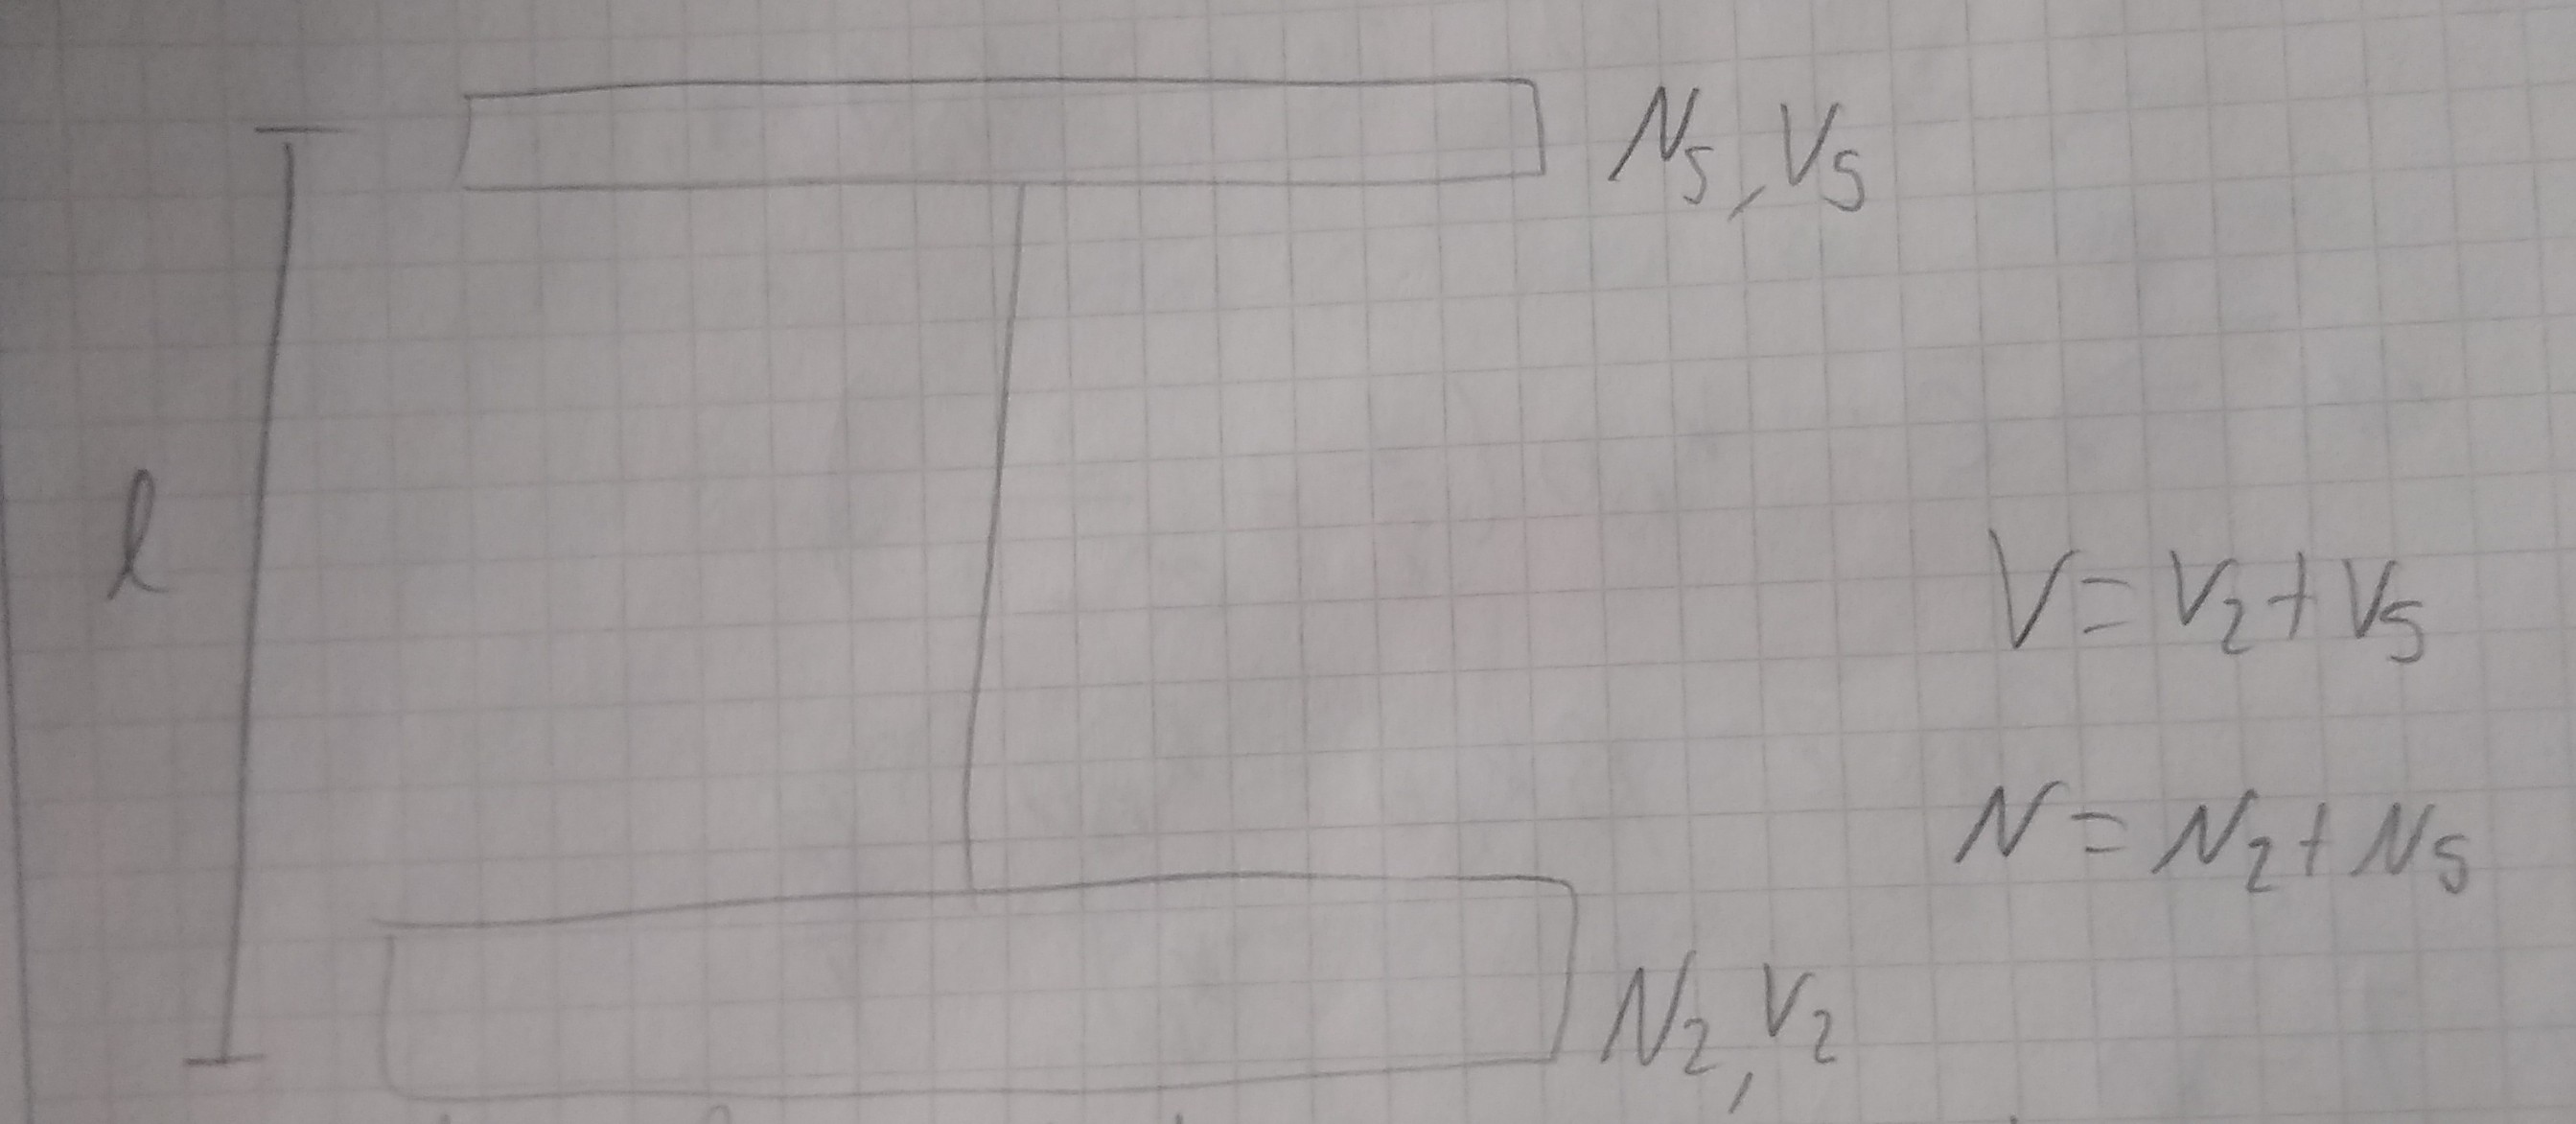
\includegraphics[width=0.95\textwidth]{sistema_fisico_5.jpg}
  \end{center}
\end{figure}
Para este sistema si la razón entre la energía potencial gravitational de las partículas contenidas en el subsistema superior con respecto a la energía térmica del gas es exactamente igual a $ \ln 2  $, encuentre la frecuencia $ \rho_5/\rho_3 $ 
\begin{gather*}
   \rho_5 = \rho_3 e ^ {- mgl / \kappa_B T } = \rho_I e ^ {-x }, \qquad \text{Con } x = \frac{m g l }{\kappa_B } \\
   x = \ln 2 \quad \rightarrow \quad \rho_3 = \rho_I e ^ {-\ln 2 } = \frac{\rho_I }{ e ^ {\ln 2 }} = \frac{\rho_I }{2 } \\
   T = \frac{m g l }{\kappa_B \ln 2 } \qquad \qquad \frac{\rho_3 }{\rho_5 } = \frac{1}{2}
\end{gather*}

\subsection{Sistema físico 1 }
Hay Indistinguibilidad 
\begin{gather*}
  Q_1 = \displaystyle\sum_{i = 1 }^{2 } e ^ {- \beta\epsilon_i } = e ^ {x } + e ^ {-x }\\ 
  x = \frac{1}{2} \ln 4 = \ln 2 \quad \rightarrow \quad  Q_1 = e ^ {\ln 2 } + \frac{1}{e ^ {\ln 2 }} = 2.5  \\
  Q_N = \frac{1}{N! } (Q_1)^N = \frac{1}{N! } (2.5)^N \\
  A = - \frac{1}{\beta} \ln Q_N = - \kappa_B  T \ln \left[\frac{1}{N! } (2.5)^N \right] = \frac{2\epsilon }{\ln 4 }  [N \ln N - N - N \ln (2.5  )] \\
  A = \frac{2 }{\ln 4 }N \epsilon \left[\ln \frac{N }{2.5 } - 1 \right]\\
   E = - \frac{3 }{2}N \epsilon
\end{gather*}


\end{document}
